\documentclass[a4paper,12pt,oneside]{article}
\usepackage{amsmath,amssymb}
\usepackage{listings}
\usepackage{latexsym}
\usepackage{pdfpages}
\usepackage{graphicx}
\usepackage{graphics}
\usepackage{url}
\usepackage{array}
\usepackage{float}
\usepackage[top=1in,bottom=1in,left=1.25in,right=1.25in]{geometry}
\bibliographystyle{ieeetr}
\title{Google Summer of Code 2014 : Performance Optimization with VOLK}
\date{\today}
\author{Abhishek Bhowmick\\ abhowmick22@gmail.com\\ \\Potential Mentors : Nathan West, Florian Kaltenberger}


\begin{document}
\maketitle
\tableofcontents
\newpage
\section{Introduction}
GNU Radio \cite{gnuradio} is a software development toolkit that can be used to implement software defined radios using commodity hardware. The signal processing blocks it provides are mostly run on general purpose processors, and performance is a key metric for the implementations on various architectures. With this in mind, GNU Radio includes VOLK, which is a library of kernels that utilize vector SIMD extensions to popular architectures (SSE, AVX, AVX2, FMA, ARM Neon). Current VOLK kernels target stock operations such as vector multiply, conjugate, dot product etc, but various benchmarking studies have shown that more complex kernels deliver better runtime performance \cite{volk-benchmark}.   

\section{Proposal}

The objectives of the project are to enhance the functionality of the VOLK library with complex kernels and advanced ISA support. First, AVX/AVX2 implementations will be developed for the current VOLK kernels, and turbo encoder/decoder blocks from OpenAirInterfaces \cite{openair} will be ported to VOLK. Next, new kernels will be developed to accelerate blocks such as the in-tree receiver OFDM implementation, ATSC 2.x, DVB-T. These new kernels will be identified based on profiling studies, to accelerate performance bottlenecks. Also, vectorized support will be developed for transcendental functions such as exp, log10, atan2f.

\section{SIMD extensions}

AVX expands SSE instructions to 256 bit and also includes 3-operand fused multiply and accumulate instructions (FMA). These can be used to speed up operations like dot products, matrix operations, convolution etc. Its extension on Haswell chips, namely AVX2, include newer features like 3-operand general purpose bit manipulation, gather loads and integer vectors. These new features alongwith wider registers can be used with good benefits. 

\section{OpenAirinterfaces and Existing Kernels}

\subsection{Porting code from OpenAirInterfaces}
\label{sec:openair}
OpenAirInterfaces~\cite{openair} already has SIMD optimized (SSE4) Turbo encoder/decoder and Viterbi encoder/decoder blocks for LTE~\cite{lte} and IEEE 802.11~\cite{802.11} standards. The objective is to write generic, aligned and unaligned VOLK wrappers for these blocks, followed by an upgrade to AVX2. The code is licensed under GPLv2 and hence can be ported to GNU Radio. The source code for these blocks may be viewed under \url{https://svn.eurecom.fr/openair4G/trunk/openair1/PHY/CODING}. The relevant vectorized codes are 3gpplte\_sse.c (LTE Turbo encoder), 3gpp\_lte\_turbo\_decoder\_sse.c (LTE turbo decoder), viterbi.c (802.11 Viterbi decoder) and viterbi\_lte.c (LTE Viterbi decoder).

\subsection{Old kernels}
\label{sec:old-kernels}
Based on the usage of VOLK kernels in various GNU Radio blocks~\cite{volk-stats} and particularly in applications like digital TV (ATSC, DVB-T), OFDM etc, the following kernels were identified for upgrading to AVX(2).

\begin{table}[h]
\centering
\begin{tabular}{ >{\itshape}p{7.7cm} | >{\itshape}p{6.3cm} }
\hline 
\textnormal{\bfseries Will do} & \textnormal{\bfseries Will do given time} \\ \hline \hline
volk\_32fc\_32f\_dot\_prod\_32fc, volk\_32f\_x2\_dot\_prod\_32f ... & volk\_32f\_convert\_64f, volk\_8i\_s32f\_convert\_32f ... \\ \hline 
volk\_32fc\_x2\_multiply\_32fc, volk\_32f\_x2\_multiply\_32f ... & volk\_32fc\_deinterleave\_64f\_x2, volk\_32fc\_deinterleave\_imag\_32f ... \\ \hline
volk\_32fc\_conjugate\_32fc & volk\_32fc\_magnitude\_squared\_32f \\ \hline
volk\_32fc\_x2\_multiply\_conjugate\_32fc & volk\_32fc\_s32fc\_x2\_rotator\_32fc \\ \hline
volk\_32fc\_s32f\_x2\_power\_spectral\_density\_32f \\ \hline
\end{tabular}
\caption{Classes of volk kernels identified for updating}
\label{tab:table1}
\end{table}

\section{Preliminary Profiling and New Kernels}
\label{sec:profiling}
Some preliminary profiling was done for the example OFDM implementation to identify performance bottlenecks. Figure~\ref{fig:1} identifies the most computationally intense blocks in OFDM Rx through a Control Flow Graph. 

\begin{figure}[h] 
\centering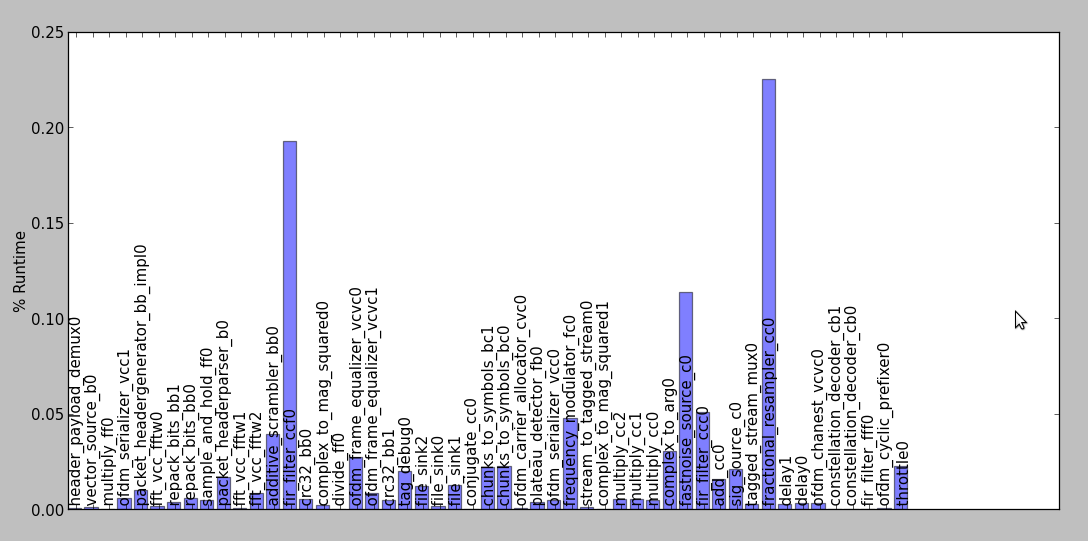
\includegraphics[width=5in]{figure/ofdm_rx.png}
\caption{Percentage runtime of different blocks in OFDM RX example \label{fig:1} }
\end{figure}

Oprofile \cite{oprofile} was used to further identify the C++ routines within these blocks that were processor heavy. For instance, the {\it fir\_filter\_ccf} and {\it fir\_filter\_ccc} blocks spent a lot of time in their respective filter() methods, that were already seen to have some vectorization with the {\it volk\_32fc\_32f/x2\_dot\_prod\_32fc\_a} kernels. AVX2 support and better vectorization can be used to target these regions. Similarly, the {\it work()} methods of {\it fractional\_resampler\_cc}, {\it additive\_scrambler\_bb} and {\it ofdm\_frame\_equalizer\_bb} are good candidates for vectorization. Also, profiling was carried out for the {\it qa\_atsc} test in gr-atsc module, which revealed that Viterbi decoder/encoder, convolutional interleaver/deinterleaver were most CPU-hungry operations.

\subsection{New Kernels}

Based on the profiling and initial discussions with GNU Radio community, following algorithms were identified for implementation as potential VOLK kernels:

\begin{itemize}
\item \textbf{OFDM Frame detection}: Current timing and frequency synchronization is done using Schmidl-Cox algorithm \cite{schmidl-cox}. The pre-FFT timing acquisition and fine frequency offset correction will be developed into a single kernel.
\item \textbf{OFDM Equalizer}: This kernel will incorporate channel estimation based on pilot symbols and DFE equalization.
\item \textbf{Viterbi Decoder, Trellis Encoder} : These were the among the most intensive blocks in ATSC loopback test. Viterbi decoder was also shown to be the most cycle hungry block in out-of-tree DVB-T implementation by Bogdan Diaconescu \cite{dvbt}. We can potentially adapt the Viterbi encoder/decoder from OpenAirInterfaces into VOLK kernels for usage in ATSC, DVB-T.
\item \textbf{Transcendental functions}: Operations like log, atan, exp, sin, cos etc.
\item \textbf{Convolutional interleaver/deinterleaver}: Data interleaving and deinterleaving were also seen to be computationally hungry in the profiling of ATSC. This will be attempted if time permits. 
\item \textbf{Miscellaneous}: Detailed profiling similar to Section~\ref{sec:profiling} is bound to reveal performance bottlenecks that can be addressed with new kernels. Some operations that were already identified include fractional resampler, fir filter, additive scrambler etc. Identifying and accelerating such operations will be attempted following detailed discussions with mentors and if time permits.
\end{itemize}

%\section{OFDM Receiver}
%Orthogonal Frequency Division Multiplexing is a method for encoding digital data on multiple carrier frequencies that are orthogonal to each other. In an OFDM receiver, the signals received from channel are down-converted, filtered, sampled and digitised. An FFT block converts these samples back into the frequency domain. The parallel streams from the FFT are then decoded into symbols using symbol detectors and serialized to get back the original data stream. \\
%
%\subsection{Frame synchronization}
%The synchronization block is needed to detect the beginning of the symbol and correct fine carrier frequency offset. The benchmark OFDM\_rx implements the Schmidl Cox Frequency/Timing Synchronization \cite{schmidl-cox}, which relies on a two-symbol training sequence, placed at the beginning of a frame. In the current implementation, symbol timing is done in the {\it ofdm\_sync\_sc\_cb} block while coarse frequency offset calculation is done in {\it chanest\_vcvc}. As both these operations are similar in nature, a new cross-correlation kernel will be developed to accelerate them.
%Another promising direction is to implement Awoseyila's method \cite{awoseyila} that uses only one training symbol to achieve time-frequency synchronization entirely in the time domain, that gives it the benefits of low complexity and fast convergence. As all processing is done in the time domain, we can combine the split frequency synchronization in the current OFDM implementation into a single frame synchronization kernel. 
%  
%\subsection{Channel Estimation}
%The {\it ofdm\_chanest\_vcvc} block does the channel estimation and coarse frequency offset, attaches this information as tags to the data symbols, strips the synchro symbols and passes the stream along. The current implementation employs a least square (LS) estimator with linear interpolation between alternate subcarriers - an MMSE estimator or higher order interpolation will be used for better performance \cite{channel-estimator}, this will require volk kernels for matrix operations. 
%
%\subsection{Equalization}
%New kernels as identified in Section~\ref{sec:profiling} will be developed to accelerate the current simple DFE equalizer. A new MMSE-DFE equalizer \cite{mmse-equalizer} will be implemented to improve performance in adverse channel conditions.

\section{Deliverables}
The following is a list of the deliverables which may be subject to change following discussions with mentors. 
\begin{itemize}
\item Deliverable 1: Upgrade existing VOLK kernels as outlined in Section~\ref{sec:old-kernels} to have AVX/AVX2 proto-kernels.
\item Deliverable 2: Port Turbo and Viterbi encoder/decoder for LTE/802.11 from OpenAirInterfaces to VOLK. This will comprise writing generic versions of these blocks, creating volk wrappers and also developing proto-kernels for AVX/AVX2. This will potentially yield Viterbi and Turbo FEC volk kernels that may be re-used by other applications.  
\item Deliverable 3: Develop new VOLK kernels for OFDM frame detection, OFDM equalizer. In addition to performance, high reconfigurability and portability to other applications such as WLAN, DVB-T, DAB etc will be key concerns.  
\item Deliverable 4: Vectorize functions like exp, log, atan, sin, cos.  
\item Deliverable 5: Detailed documentation, QA tests for the above. 
\item Deliverable 6: (Variable) If time permits, target additional operations such as data interleaving, resampling, filtering, PSK sync. Potential operations to be accelerated will be identified before GSoC begins. Their implementation will be done within GSoC period if time permits, or after program completion as part of continuing association with the community.
\end{itemize}

\section{Hardware required}

A Haswell processor from Intel will be required for developing kernels with AVX2 support. Also, a USRP board might be needed for testing real-time capabilities of applications like ATSC and DVB-T. 

\section{Schedule/Availability}
A tentative schedule for the project is as follows: 
%\begin{itemize}
%\item \textbf{Pre GSoC phase}: Get familiar with AVX/AVX2, programming with SIMD intrinsics, error correcting codes.   
%\item \textbf{19 May - 23 May} (1 week): Examine the source code, detailed profiling studies, discussions with mentor on design of new kernels.
%\item \textbf{26 May - 6 June} (2 weeks): Upgrade VOLK kernels from Section~\ref{sec:old-kernels} to AVX/AVX2. 
%\item \textbf{9 June - 20 June} (2 weeks): Code OFDM Frame detection kernel.
%\item \textbf{23 June - 27 June} (1 week): Mid-term evaluations, add documentation, testing, benchmarking.
%\item \textbf{30 June - 11 July} (2 weeks): Port OpenAirInterfaces blocks to VOLK and upgrade to AVX2.
%\item \textbf{14 July - 18 July} (1 week): Functional tests, benchmarking, documentation.
%\item \textbf{21 July - 1 Aug} (2 weeks): Code OFDM frame equalizer kernel. 
%\item \textbf{4 Aug - 8 Aug} (1 week): Vectorize exp, log, trig functions.
%\item \textbf{11 Aug - 15 Aug} (1 week): Write tests, bug fixes, clean code, add documentation.
%\end{itemize}

\begin{table}[H]
\centering
\begin{tabular}{>{\bfseries}p{3.8cm} p{10.2cm}}
\hline
Pre GSoC phase & Get familiar with AVX/AVX2, programming with SIMD intrinsics, detailed profiling to identify performance bottlenecks, engage with the community. \\ 
19 May - 23 May \par \textnormal{(1 week)} & Finalize kernels to be implemented, formally define functional specifications \\
26 May - 6 June \par \textnormal{(2 weeks)} & Upgrade VOLK kernels from Section~\ref{sec:old-kernels} to AVX/AVX2. \\
9 June - 20 June \par \textnormal{(2 weeks)} & Code OFDM Frame detection kernel. \\ 
23 June - 27 June \par \textnormal{(1 week)} & Mid-term evaluations, add documentation, testing, benchmarking. \\ 
30 June - 11 July \par \textnormal{(2 weeks)} & Port OpenAirInterfaces channel coding blocks to VOLK and upgrade to AVX/AVX2. \\ 
14 July - 18 July \par \textnormal{(1 week)} & Functional tests, benchmarking, documentation. \\ 
21 July - 1 Aug \par \textnormal{(2 weeks)} & Code OFDM frame equalizer kernel. \\ 
4 Aug - 8 Aug \par \textnormal{(1 week)} & Vectorize exp, log, trig functions. \\ 
11 Aug - 15 Aug \par \textnormal{(1 week)} & Write tests, bug fixes, clean code, add documentation. \\ 
\hline
\end{tabular}
\end{table}

My availability is as follows:

\begin{itemize}
\item \textbf{Expected hrs/week}: 40 hours per week
\item \textbf{Off period}: Approx. 5 blackout days, not contiguous. Lost time will be compensated appropriately.
\item \textbf{Other commitments}: Possibly one online course (not finalized yet), with 10-15 hrs/week requirement.
\end{itemize}

\section{Background}
I finished my B.Tech in Electrical Engineering from IIT Bombay, India in 2013 and spent the following period working as a research assistant at Carnegie Mellon University, USA. A paper I co-authored based on this work was accepted for publication at ISCA 2014 (International Symposium on Computer Architecture). I am currently working as a research staff at IIT Bombay. I will join a Masters program in Computer Science in August 2014 (school yet to be finalized). My primary research interest is Computer Architecture and I have undergraduate level experience in Signal Processing (courses on Signal/Systems, Communication Systems and Digital Communications). I have significant experience coding in C++ and written some code in Python. I also have some experience in x86 assembly and hence would be comfortable with any ASM programming that might be required. You may find some code that I have written previously, on my github: \url{https://github.com/abhowmick22}. You may find information about my research and my CV at my personal website: \url{https://sites.google.com/site/abhowmick22}.  

\subsection{Why GSoC?}

My primary motivation is to develop code for a large software project and be part of an open source community - this will help my career objectives. I won't receive any university credits for this work - I am participating in order to get experience working on a project with a large codebase, and the whole cycle of software development, testing, maintenance. 

\subsection{Why GNU Radio?}

Working with GNU Radio allows me to leverage my electrical engineering background and gives me an opportunity to apply concepts learned in college to real-life scenarios. Also, my interest in developing software for parallel architectures drove me to choose software optimization using SIMD extensions.

\subsection{What after GSoC?}

Post GSoC, I wish to continue developing more kernels for the VOLK library - finishing off the kernels that were identified but not completed within the timeline of GSoC. I already have some experience with GPU programming, and continuing the work on VOLK will give me significant experience with SIMD programming - such a skill set aligns perfectly with my interest in parallel computing. I am also interested in going beyond vectorization to develop signal processing blocks, however I didn't include it in my proposal keeping in mind the time constraints. As I will be pursuing a Masters degree, I will talk with mentors to work out a realistic plan for continuing my association.
 
\section{Conclusion}
I would like to acknowledge Nathan West, Martin Braun, Tom Rondeau, Bogdan Diaconescu and the entire community for helping me get started with GNU Radio and advising me on the proposal. I sincerely hope that I get to be a part of the GNU Radio community, either through GSoC or otherwise. 

\bibliography{ref.bib}

\end{document}
 
